
\documentclass{include/thesisclass3}

\SelectLanguage{ngerman}
\usepackage{float}


% Titlepage settings
\newcommand{\praktikum}{Praktikum moderne Physik}
\newcommand{\autora}{Jens Schäfer}
\newcommand{\autorb}{Jan van der Linden}
\newcommand{\maila}{ugecd@student.kit.edu}
\newcommand{\mailb}{jan.vdlinden95@gmail.com}
\newcommand{\topic}{Landé factor of the muon}
\newcommand{\ptime}{12. Juni 2017}


% Shortcuts
\newcommand{\cc}{\cdot}
\newcommand{\rk}{\rangle}
\newcommand{\lk}{\langle}
\newcommand{\df}{\rightarrow}
\newcommand{\la}{\lambda}
\newcommand{\dd}{{\rm d}}
\newcommand{\ehm}{\mathbbm{1}}
\newcommand{\p}{\partial}
\newcommand{\soll}{\overset{!}{=}}
\newcommand{\D}{\Delta}
\newcommand{\eps}{\epsilon}
\newcommand{\vektor}[3]{\begin{pmatrix} #1 \\ #2 \\ #3 \end{pmatrix}}
\newcommand{\vektorz}[2]{\begin{pmatrix} #1 \\ #2 \end{pmatrix}}
\newcommand{\Mat}[9]{\begin{pmatrix}#1&#2&#3\\#4&#5&#6\\#7&#8&#9\end{pmatrix}}
\newcommand{\Matz}[4]{\begin{pmatrix}#1&#2\\#3&#4\end{pmatrix}}
\newcommand{\e}[1]{\,\si{#1}}
 


\begin{document}

	\FrontMatter
	% coordinates for background border
\newcommand{\diameter}{20}
\newcommand{\xone}{-15}
\newcommand{\xtwo}{160}
\newcommand{\yone}{15}
\newcommand{\ytwo}{-253}




\begin{titlepage}
    % background border
    \begin{tikzpicture}[overlay]
    \draw[color=gray]
            (\xone mm, \yone mm)
      -- (\xtwo mm, \yone mm)
    arc (90:0:\diameter pt)
      -- (\xtwo mm + \diameter pt , \ytwo mm)
        -- (\xone mm + \diameter pt , \ytwo mm)
    arc (270:180:\diameter pt)
        -- (\xone mm, \yone mm);
    \end{tikzpicture}



    % KIT image and sign for faculty of physics
    \begin{textblock}{10}[0,0](4.5,2.5)
        
\includegraphics[width=.25\textwidth]{include/kitlogo.pdf}
    \end{textblock}
    

    % horizontal line
    \begin{textblock}{10}[0,0](4.2,3.1)
        \begin{tikzpicture}[overlay]
        \draw[color=gray]
                (\xone mm + 5 mm, -12 mm)
          -- (\xtwo mm + \diameter pt - 5 mm, -12 mm);
        \end{tikzpicture}
    \end{textblock}



    % begin of text part
    \changefont{phv}{m}{n}    % helvetica
    \centering



    % thesis topic (en and ge)
    \vspace*{3cm}
    \Huge\praktikum\\



    % author name and institute
    \vspace*{5cm}
    
    \huge\topic\\






    % examiners (Referenten)
    \vspace*{3cm}
    \Large
    \begin{center}
        \begin{tabular}[ht]{l c l } 
  \autora & \hfill & \textit{\maila} \\
\autorb & \hfill & \textit{\mailb} \\
        
        \end{tabular}
    \end{center}



    % working time
    \vspace{2cm}
    \begin{center}
        \large{Durchgeführt am}: \ptime
    \end{center}



    % lowest text blocks concerning the KIT
    \begin{textblock}{10}[0,0](4,16.8)
        \tiny{KIT -- Universität des Landes Baden-Württemberg und nationales %
              Forschungszentrum in der Helmholtz-Gemeinschaft}
    \end{textblock}
    \begin{textblock}{10}[0,0](14,16.75)
        \large{\textbf{www.kit.edu}}
    \end{textblock}
\end{titlepage}

	\tableofcontents                  
	\newpage
	\MainMatter

%Protokollstart

\chapter{Theoretical Background}

In this experiment the lifetime of a muon is to be determined, as well as its Landé factor.
\todo{...}% what is dat?

\section{Cosmic muons}
Primary cosmic radiation consists mainly of protons (85\%), $\alpha$ particles and photons.
When entering the atmosphere secondary particles are induced by interacting with the matter in the atmoshpere.
A strong interaction with air molecules induces the production of pions, protons and neutrons.
Due to the short halflife of pions, they do not reach the earth, but rather convert either into a pair of photons (in the case of the neutral pion) or into a charged lepton and its corresponding anti-neutrino ($\pi^\pm ~\df~ \mu^\pm + \nu_\mu/\bar{\nu}_\mu$).
The muons have a higher range in comparison with the electrons, because they are far heavier.
Also, due to the high energies of the cosmic radiation, also the muons have very high energies and are therefore ultrarelativistic.
As the mean lifetime of a muon is approximately $\tau = 2.2\cc10^{-6}\e{s}$ they should in gerneral not be able to reach earth.
The muons are however ultrarelativistic, which enables them to reach earth, because the lifetime holds for the restframe of the muon, which translates to $\tau_E = \gamma \tau$ in an observers frame.
Therefore even muons with energies of $10\e{GeV}$ are able to travel over $60\e{km}$ or more.

In matter, high energy muons lose energy mainly by bremsstrahlung; the emission of photons.
In lower energy ranges (under GeV) they also lose notable amounts of energy from ionization processes or coulomb interaction.
Furthermore, negative muons $\mu^-$ get caught by atoms and get absorbed into the nucleus by interacting via the weak force.
Thus, the lifetime of $\mu^-$ reduces a lot when passing through matter, which results in the main part of the cosmic muon radiation to consist of positive muons $\mu^+$.

At the end of the lifetime of the positive muons they usually convert into positrons via $\mu^+ ~\df~e^+ + \mu_e + \bar{\nu}_\mu$. 
\section{Muon polarization}
%In certain energy intervals, the momentum of muons is polarized, because of the parity violation of the weak interaction.
As pions carry spin $0$ and the neutrino must have negative chirality due to its velocity/vanishing mass the antimuon is forced by conservation of spin and momentum to have negative chirality aswell (maximum parity violation of weak interaction only permits particles of negative and antiparticles of possitive chirality).
Now, the muons also have different energies, depending on the direction of emission from the pion.
If the muon is emitted in the direction of travel in the rest frame of the decaying pion, it has a higher energy than the muons emitted in the opposite direction. For a muon emitted against the direction of travel, a negative polarization is expected, whereas a positive polarization is expected for the muons emitted in the direction of travel.
Observing a certain energy interval there are muons with equal energys but different polarization depending if it was emitted by low-energy pions in direction of travel or by high-energy pions in opposite direction. In a matter of fact there is a non-equal distribution of pions in different energy scales. Therefore, there will be a polarization of approximately $P=-\frac{1}{3}$ observable, if a energy sensitive measurement will be performed at purpendicular incidence angle.

\section{Evidence of muon decay}
To measure a decaying muon the conversion into a positron $e^+$ and two invisible neutrinos has to be observed.
The double differential cross section for this process is given by
$ \frac{\d N}{\d \eps \d \Omega} = \frac{\eps}{2\pi} \left[ (3-2\eps) - P(1-2\eps)\cos\theta\right] \equiv a(1 + b \cos\theta) $
Here, $\eps$ denotes the relative energy $\eps = E/E_{max}$, where $E_{max} = m_\mu/2$, and $\theta$ denotes the angle between the spin of the incident muon and the momentum of the positron. 
The polarization of the muon is called $P$.

\section{Landé factor of the muon}
With a magnetic field applied, the muon precess around the direction of $B$ with frequency $\omega = \gamma B$ where $\gamma$ is the gyromagnetic ratio
\[ \gamma = g \frac{\mu_B}{\hbar}, ~~~\mu_B = \frac{e\hbar}{2m}\]
For the muon, the Bohr magneton is equivalent to $\mu_B = 4.5\cc10^{-26}\e{\frac{J}{T}}$ and $g$ is the Landé factor of the muon.
This factor can be measured through measurement of the precession frequency of a free particle in a magnetic field, such that
\[ g = \frac{\hbar \omega}{\mu_B B}\]

\section{Principle of measurement}
By observing the differenz in time of the muon decellerating in the observer and the appearence of the positron the mean lifetime can be calculated
\begin{equation}
N(t)=N_0\,e^{-t/\tau}
\end{equation}
Therefore three szintillators are layerd with a cupper absorber inbetween the last two. Each layer is about 2.5cm thick. With trigger hardware only muons passing through layer 1 and 2 but not through 3 are counted. 
For the Landé factor the precission frequency has to be measuered. Therefore the absober material is penetrated with the magnetic field B and again the mean lifetime gets observed but just on a decent ancle $\theta$. The ratio of decaying myons is now modulated by the precission and the ancle transforms into $\omega t$ therefore the mean lifetime goes to 
\begin{equation}
N(t)=K\cdot e^{ -t/\tau } \cdot [ 1+\bar A \cdot \cos(\omega t + \delta )]\label{n(t)}
\end{equation}

\section{Analysis}
The data used to calculate are measurements taken over the last two years. After adding them all together a rawdata is build

\begin{figure}[ht]
	\begin{center}
		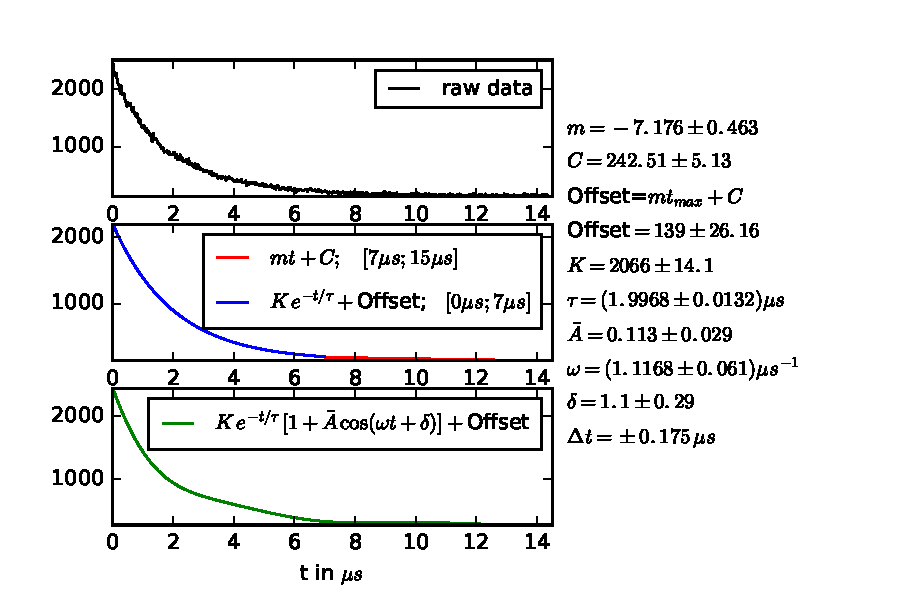
\includegraphics[scale=1.2]{images/plot.pdf}
		\caption{Rawdata and three fits via the second methond are displayed aswell as the fitted functions and parameters}
		\label{method2}
	\end{center}
\end{figure}
To fit the function \ref{n(t)} it is possible to do a fit with six parameters (first methode) but also to seperate the Data into two sets where the first set clearly behaves exponential and the second linear. By fitting each section itself single Parameter could be extracted more certain. \\
The division took place after 0.7$\e{\mu s}$. The second area gives a linear function, its lowest point is interpreted as the offset, originated by random noises in the detector. With knowledge of this offset the next fit in exponential shape could be done. Therefore the first area is used and the parameters K and $\e{\tau}$ were calculated. After these steps K, $\e{\tau}$ and the offset are known and \ref{n(t)} reduces to three unknown parameters. The last step fits the remaining ones over the whole dataset. All fits and results are deployed in image \ref{method2}. The errors inside the image are results of the fitting methode and the datarange missing the uncertainity in the other parameters aswell as in time. To calculate the real error an errorpropagation has to be made wich results in a slightly different result in $\tau$ and the same error in $\omega$:
\begin{align}
&\e{Lifetime} &\tau=(0.1997\pm 0.0012)\e{\mu s}\\
&\e{Landé-factor} &g=(a\pm b)
\end{align}

%\chapter{Experiment and Analysis}

\end{document}
